\documentclass{standalone}

% graphics
\usepackage{tikz}
\usepackage{pgfplots}
\usepackage{siunitx}

\begin{document}

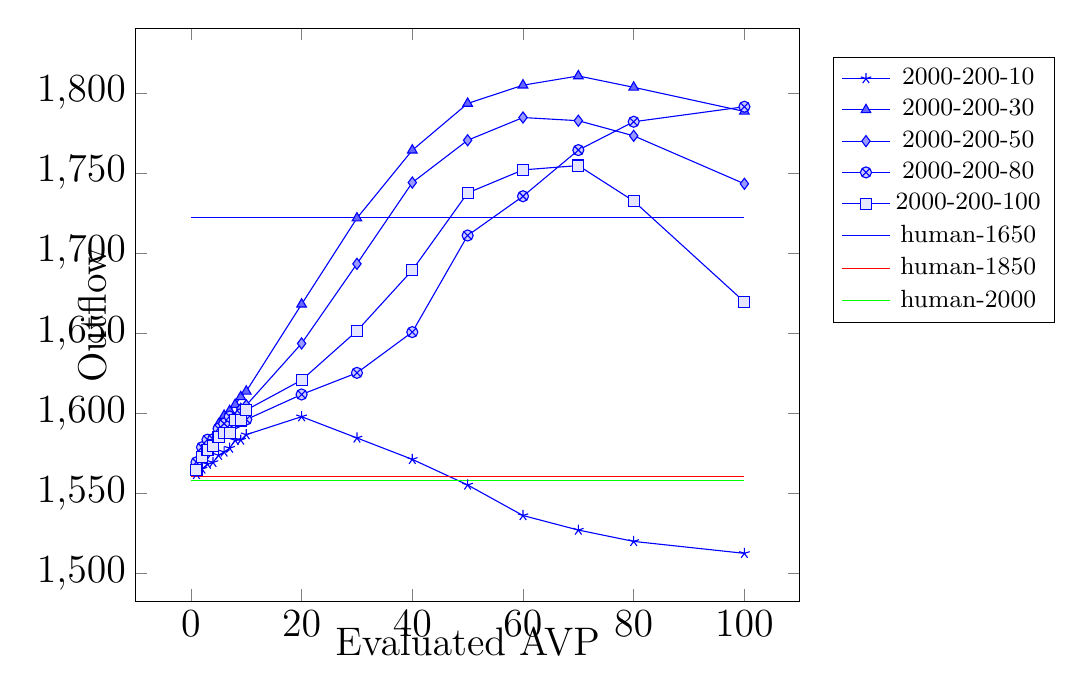
\begin{tikzpicture}[scale=1]
  \pgfplotsset{
      scale only axis,
      every x tick label/.append style={font=\Large},
      every y tick label/.append style={font=\Large},
	legend style={at={(1.05,0.95)},anchor=north west}
  }

\pgfplotscreateplotcyclelist{mycolorlist}{%
	blue,every mark/.append style={fill=blue!80}, mark=star, error bars/.cd, y dir=both, y explicit\\%
	blue,every mark/.append style={fill=blue!60}, mark=triangle*, error bars/.cd, y dir=both, y explicit\\%
	blue,every mark/.append style={fill=blue!40}, mark=diamond*, error bars/.cd, y dir=both, y explicit\\%
	blue,every mark/.append style={fill=blue!20}, mark=otimes*, error bars/.cd, y dir=both, y explicit\\%
	blue,every mark/.append style={fill=blue!10}, mark=square*, error bars/.cd, y dir=both, y explicit\\%
	red,densely dashed,every mark/.append style={solid,fill=red!80}, mark=star, error bars/.cd, y dir=both, y explicit\\%
	red,densely dashed,every mark/.append style={solid,fill=red!60},mark=triangle*, error bars/.cd, y dir=both, y explicit\\%
	red,densely dashed,every mark/.append style={solid,fill=red!40},mark=diamond*, error bars/.cd, y dir=both, y explicit\\%
	red,densely dashed,every mark/.append style={solid,fill=red!20}, mark=otimes*, error bars/.cd, y dir=both, y explicit\\%
	red,densely dashed,every mark/.append style={solid,fill=red!10}, mark=square*, error bars/.cd, y dir=both, y explicit\\%
	green!40!black, dashed,every mark/.append style={solid,fill=green!80}, mark=star, error bars/.cd, y dir=both, y explicit\\%
	green!40!black, dashed,every mark/.append style={solid,fill=green!60},mark=triangle*, error bars/.cd, y dir=both, y explicit\\%
	green!40!black, dashed,every mark/.append style={solid,fill=green!40},mark=diamond*, error bars/.cd, y dir=both, y explicit\\%
	green!40!black, dashed,every mark/.append style={solid,fill=green!20},mark=otimes*, error bars/.cd, y dir=both, y explicit\\%
	green!40!black, dashed,every mark/.append style={solid,fill=green!10},mark=square*, error bars/.cd, y dir=both, y explicit\\%
	black, dashed,every mark/.append style={solid,fill=green!80}, mark=star, error bars/.cd, y dir=both, y explicit\\%
	black, dashed,every mark/.append style={solid,fill=green!60},mark=triangle*, error bars/.cd, y dir=both, y explicit\\%
	black, dashed,every mark/.append style={solid,fill=green!40},mark=diamond*, error bars/.cd, y dir=both, y explicit\\%
	black, dashed,every mark/.append style={solid,fill=green!20},mark=otimes*, error bars/.cd, y dir=both, y explicit\\%
	black, dashed,every mark/.append style={solid,fill=green!10},mark=square*, error bars/.cd, y dir=both, y explicit\\%
	}


\begin{axis}[
    legend style={font=\small},
	ylabel={\Large Outflow},
	x label style={at={(axis description cs:0.5,-0.03)},anchor=north},
	y label style={at={(axis description cs:-0.030,0.5)}, anchor=south},
	xlabel={\Large Evaluated AVP},
	cycle list name=mycolorlist
]

\addplot table [x=a, y=b] {
a	 b	 c
1	1561.75	18.33
2	1565.14	19.91
3	1568.16	20.49
4	1569.24	20.16
5	1573.74	18.58
6	1575.76	19.96
7	1578.17	22.33
8	1583.06	25.2
9	1583.21	23.07
10	1586.56	18.1
20	1597.79	27.08
30	1584.5	25.72
40	1571.15	32.98
50	1555.16	24.21
60	1536.08	27.92
70	1527.01	25.58
80	1519.92	29.22
100	1512.47	25.56
};
\label{2000-200-10}

\addplot table [x=a, y=b] {
a	 b	 c
1	1566.14	20.01
2	1571.83	21.59
3	1579.18	24.32
4	1584.43	22.76
5	1593.14	29.73
6	1598.51	29.32
7	1601.42	32.0
8	1605.31	27.14
9	1610.14	28.18
10	1613.63	39.37
20	1667.99	46.01
30	1721.74	47.9
40	1764.14	49.66
50	1793.34	44.19
60	1804.75	43.3
70	1810.51	33.17
80	1803.42	29.42
100	1788.37	21.97
};
\label{2000-200-30}

\addplot table [x=a, y=b] {
a	 b	 c
1	1565.57	21.02
2	1572.01	20.42
3	1574.93	22.35
4	1578.96	18.07
5	1584.94	26.08
6	1589.54	25.88
7	1596.92	27.99
8	1597.1	27.99
9	1602.72	27.16
10	1604.92	31.18
20	1643.51	37.18
30	1693.22	56.8
40	1743.95	53.01
50	1770.37	55.99
60	1784.56	39.64
70	1782.58	39.46
80	1773.14	32.93
100	1743.19	27.62
};
\label{2000-200-50}

\addplot table [x=a, y=b] {
a	 b	 c
1	1569.35	18.91
2	1578.71	22.15
3	1583.46	22.82
4	1583.75	24.92
5	1590.34	25.89
6	1593.47	24.85
7	1597.9	27.33
8	1593.72	26.02
9	1599.37	27.72
10	1595.99	31.33
20	1611.65	37.06
30	1625.15	57.34
40	1650.6	54.06
50	1710.9	63.37
60	1735.42	58.32
70	1764.22	52.0
80	1781.93	50.15
100	1791.29	36.55
};
\label{2000-200-80}

\addplot table [x=a, y=b] {
a	 b	 c
1	1564.31	19.99
2	1572.52	21.75
3	1576.98	23.11
4	1579.75	22.94
5	1585.33	24.49
6	1587.38	23.12
7	1587.67	22.6
8	1595.52	23.28
9	1595.45	24.04
10	1601.93	24.26
20	1620.61	33.03
30	1651.36	39.23
40	1689.26	42.11
50	1737.47	46.26
60	1751.87	38.97
70	1754.57	36.69
80	1732.39	30.78
100	1669.46	22.85
};
\label{2000-200-100}

\addplot[blue, samples=200] coordinates {(0,1722.200000) (100,1722.200000)};\label{human-1650}\addplot[red, samples=200] coordinates {(0,1560.380000) (100,1560.380000)};\label{human-1850}\addplot[green, samples=200] coordinates {(0,1558.120000) (100,1558.120000)};\label{human-2000}\addlegendimage{/pgfplots/refstyle=2000-200-10}
\addlegendentry{2000-200-10}
\addlegendimage{/pgfplots/refstyle=2000-200-30}
\addlegendentry{2000-200-30}
\addlegendimage{/pgfplots/refstyle=2000-200-50}
\addlegendentry{2000-200-50}
\addlegendimage{/pgfplots/refstyle=2000-200-80}
\addlegendentry{2000-200-80}
\addlegendimage{/pgfplots/refstyle=2000-200-100}
\addlegendentry{2000-200-100}
\addlegendimage{/pgfplots/refstyle=human-1650}
\addlegendentry{human-1650}
\addlegendimage{/pgfplots/refstyle=human-1850}
\addlegendentry{human-1850}
\addlegendimage{/pgfplots/refstyle=human-2000}
\addlegendentry{human-2000}


\end{axis}
\end{tikzpicture}
\end{document}
